\documentclass[12pt, oneside]{article}   	% use "amsart" instead of "article" for AMSLaTeX format
\usepackage{geometry}                		% See geometry.pdf to learn the layout options. There are lots.
\geometry{letterpaper}                   		% ... or a4paper or a5paper or ... 
%\geometry{landscape}                		% Activate for rotated page geometry
%\usepackage[parfill]{parskip}    		% Activate to begin paragraphs with an empty line rather than an indent
\usepackage{graphicx}				% Use pdf, png, jpg, or eps§ with pdflatex; use eps in DVI mode
\graphicspath{ {../figures/} }
								% TeX will automatically convert eps --> pdf in pdflatex		
\usepackage{amssymb}
\usepackage{amsmath}
\usepackage{hyperref}
\usepackage{float}
\usepackage[toc,page]{appendix}
% \usepackage[cache=false]{minted}

% Move page number down
% \setlength{\footskip}{0.001cm}
% \pagenumbering{gobble}

%SetFonts

%SetFonts


\title{%
	Movie Rating Prediction Using Artificial Neural Networks}
\author{Christopher Pyles}
\date{May 5, 2020}							% Activate to display a given date or no date

\begin{document}

\maketitle

\newpage

\tableofcontents

\newpage

\addcontentsline{toc}{section}{Abstract}
\section*{Abstract}

\newpage

\section{Introduction}

\newpage

\section{Data}

The data used in this project is from \href{https://api.tmdb.org}{The Movie Database's (TMDb) API}. The data queried covers movies released in 2018 in English, spanning many genres: 

\begin{itemize}
\item Action ($n=242$)
\item Adventure ($n=134$)
\item Animation ($n=116$)
\item Comedy ($n=566$)
\item Crime ($n=154$)
\item Documentary ($n=432$)
\item Drama ($n=746$)
\item Family ($n=147$)
\item Fantasy ($n=143$)
\item History ($n=66$)
\item Horror ($n=438$)
\item Music ($n=119$)
\item Mystery ($n=143$)
\item Romance ($n=222$)
\item Science Fiction ($n=188$)
\item TV Movie ($n=194$)
\item Thriller ($n=506$)
\item War ($n=29$)
\item Western ($n=31$)
\end{itemize}

The data, after being queried, were joined into a single table and written to a CSV file. The columns of interest are described in Table \ref{table:cols_of_interest}. After dropping rows with missing values in the columns of interest, the data contained $n=2700$ rows.

\begin{table}
\begin{center}\begin{tabular}{c|l}
\textbf{Column} & \textbf{Description} \\ \hline
\texttt{id} & \textbf{primary key}, a unique ID number for each movie \\
\texttt{adult} & whether or not the movie is R+ rated \\
\texttt{genre\_ids} & list of genre ID numbers corresponding to \texttt{genres} table \\
\texttt{original\_language} & the language that the movie was originally released in \\
\texttt{original\_title} & the title of the movie \\
\texttt{overview} & movie synopsis \\
\texttt{release\_date} & the date of first release \\
\texttt{vote\_average} & average of rating votes on a 10-point scale \\
\texttt{vote\_count} & the number of votes \\
\texttt{poster\_path} & URL path to movie poster \\
\end{tabular}\end{center}
\caption{\label{table:cols_of_interest}Column descriptions for TMDb API data (the \texttt{movies} table).}
\end{table}

\subsection{Data Cleaning}

Cleaning the data for this project, after dropping missing values, involved rounding the \texttt{vote\_average} column, cleaning the synopsis strings, joining the \texttt{genres} and \texttt{movies} tables, and converting the movie posters into 140 $\times$ 92 $\times$ 3 arrays of RGB values.

The \texttt{vote\_average} column ($\mu = 6.628$, $\sigma = 1.939$) describes the variable of interest, representing the average rating across votes for a single movie. In this analysis, this column will be transformed from a continuous variable into an ordinal variable with possible values 1 to 10 by rounding the vote average to a whole number. After rounding, the distribution of ratings is provided in Figure \ref{fig:rating_barplot}.

\begin{figure}%[H]
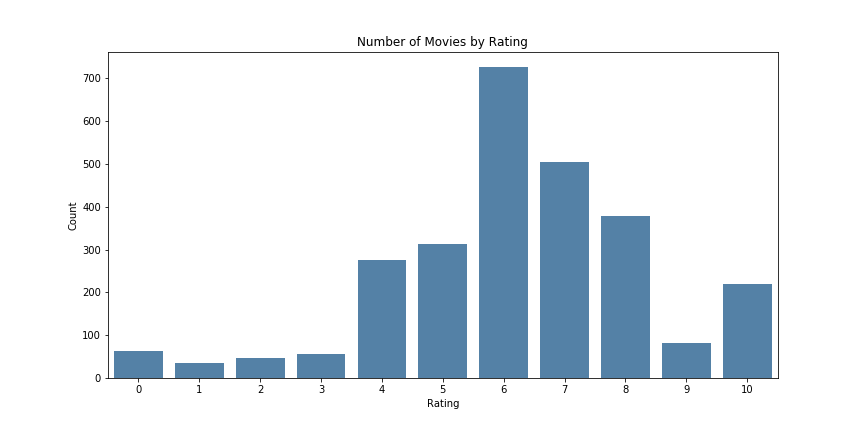
\includegraphics[width=\textwidth]{rating_barplot}
\caption{\label{fig:rating_barplot}Number of movies for each value of ratings, rounded from \texttt{vote\_average}.}
\end{figure}

To clean the movie synopses, all letters were transformed to lowercas, and any characters not matching the regex \texttt{[A-Za-z0-9 ]} were replaced with spaces.

The \texttt{genre\_ids} column is a list of genre IDs encoded as a string, so to start any empty lists, \texttt{"[]"}, were replaced with \texttt{NaN}. Then, the string were split into Python lists of IDs, and were joined with the \texttt{genres} table, so that \texttt{movies} had a column \texttt{genres} where each value is a list of genres for that movie. Figure \ref{fig:genre_barplot} shows the breakdown of movies by genre.

\begin{figure}%[H]
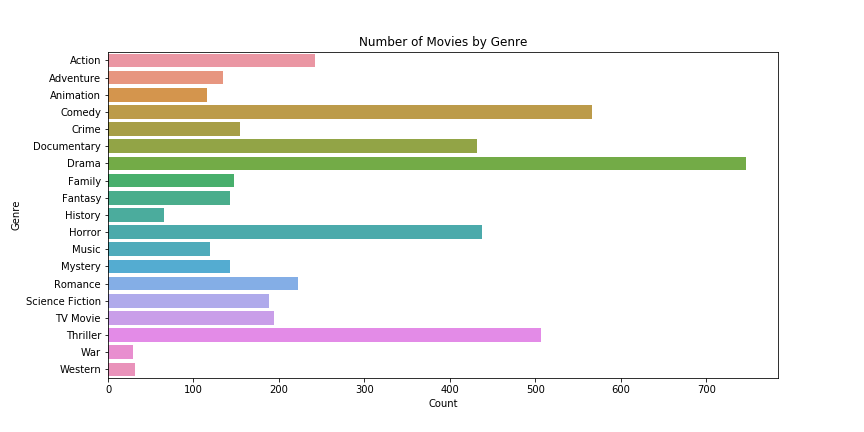
\includegraphics[width=\textwidth]{genre_barplot}
\caption{\label{fig:genre_barplot}Number of movies in each genre.}
\end{figure}

Lastly, each movie poster was downloaded from TMDb and stored as a 140 $\times$ 92 $\times$ 3 array in NumPy, stored as a .mat file. The structure of this file is analagous to a dictionary, where each key is a movie ID (as a string) and each value is the 3-D array of RGB values describing the poster.

\subsection{Exploratory Data Analysis}

Before modeling, a cursory analysis of the data yielded the interesting relationships:

\begin{itemize}

\item Figure \ref{fig:vote_count_by_rating} shows that vote count tends to increase logarithmically with rating until 8, after which it drops significantly. This demonstrates that having more votes tends to "bring down the curve."

\begin{figure}%[H]
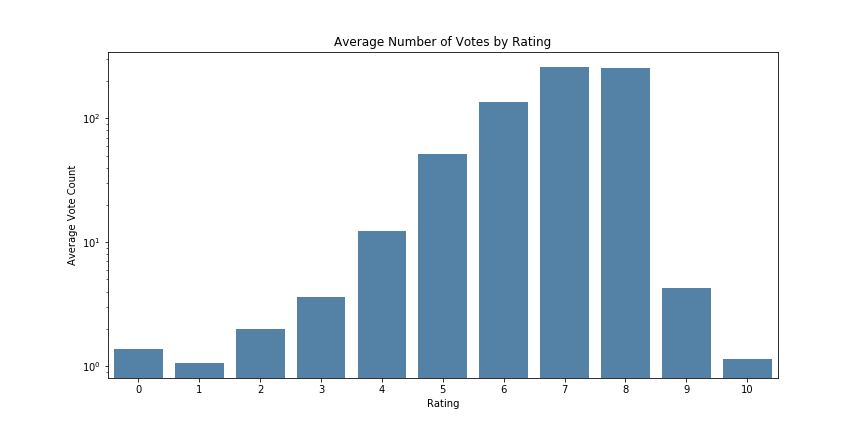
\includegraphics[width=\textwidth]{vote_count_by_rating}
\caption{\label{fig:vote_count_by_rating}Average vote count by rating.}
\end{figure}

\item There are significantly more non-adult movies than adult movies, as demonstrated in Figure \ref{fig:ratings_by_adult}. It is interesting to note that adult movies have a double-peak distribution with far less spread than do the non-adult movies.

\begin{figure}%[H]
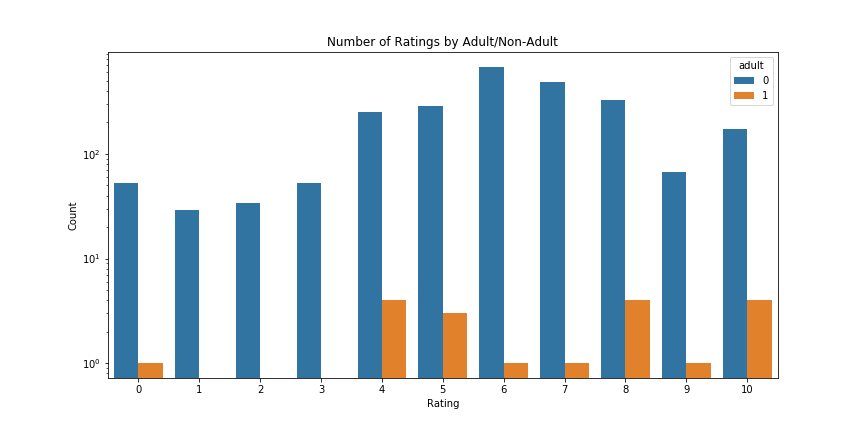
\includegraphics[width=\textwidth]{ratings_by_adult}
\caption{\label{fig:ratings_by_adult}Number of ratings by adult/non-adult.}
\end{figure}

\item Figure \ref{fig:ratings_by_genre} shows the distribution of ratings for each genre.

\begin{figure}%[H]
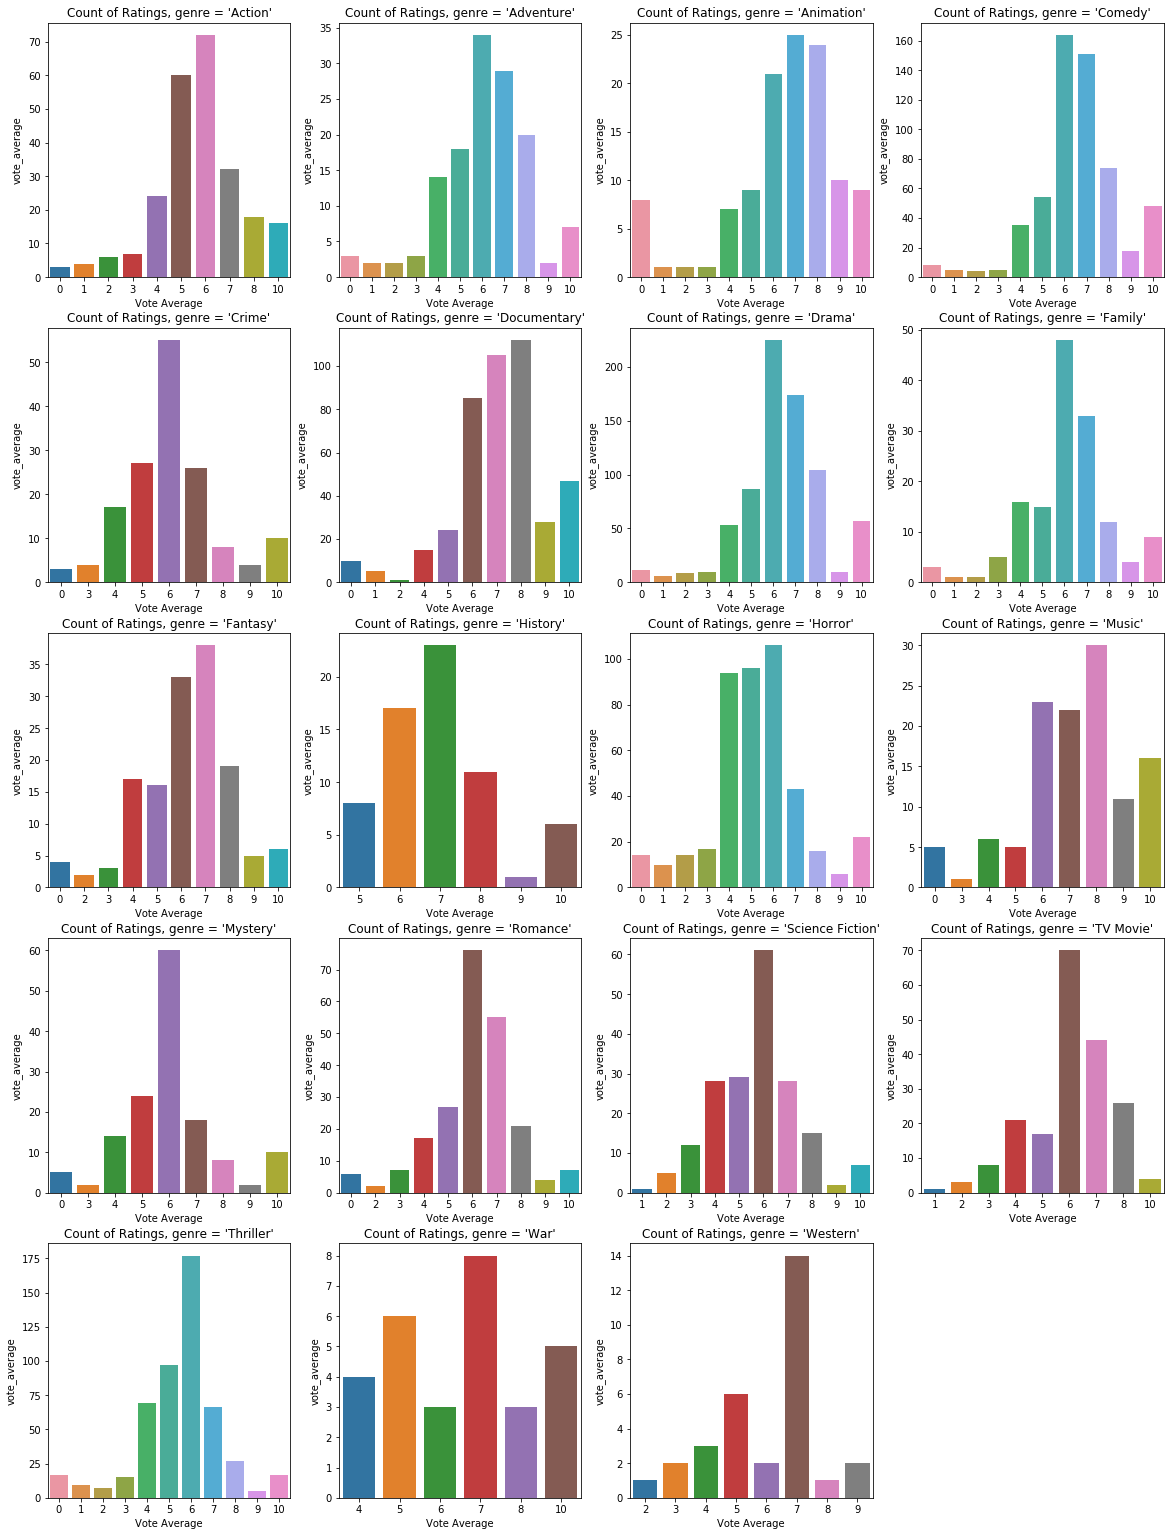
\includegraphics[height=0.9\textheight]{ratings_by_genre}
\caption{\label{fig:ratings_by_genre}Distribution of ratings by genre.}
\end{figure}

\item No discernible relationship is seen between the length of the overview and the movie's rating.

\item The distributions of ratings by release date day of week appear to be different in skew (Figure \ref{fig:ratings_dow}), indicating that this may be an important feature. No discernible relationship is seen between rating and day of month or month of release.

\begin{figure}%[H]
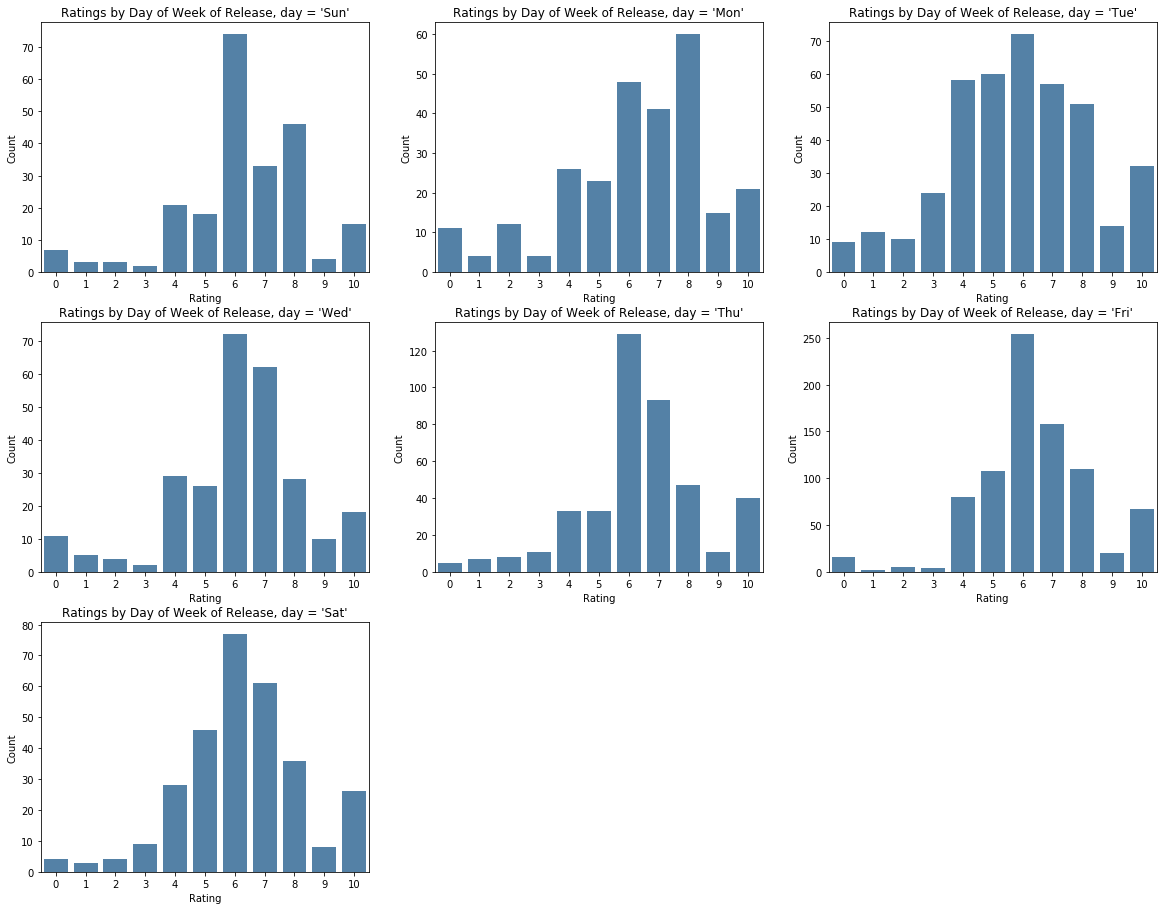
\includegraphics[width=\textwidth]{ratings_dow}
\caption{\label{fig:ratings_dow}Distribution of ratings by day of week of release.}
\end{figure}

\end{itemize}

\newpage

\section{Analysis}

\subsection{Words in Synopses}

As the first part of this analysis, the statistical significance of the presence of different words in synopses is studied using hypothesis testing. The null hypothesis for this test is that the presence of a word does not affect the average rating, and the alternative is that the presence of the word results in an increase in rating. The test statistic used here is the aboslute difference between the mean rating of movies where the word is present in the synopsis and the movies where it is not. Under the null hypothesis, the truth value of a word being present in a synopsis is shuffled for each observation, so that same number of ``present''s is obtained. Then, the test statistic is computed and the p-value is calculated as the proportion of the test statistic values that are greater than or equal to the observed value for that word. Finally, those words whose p-values indicate statistical significance are added to the movies data as one-hot features, with a 1 in their column if the word is present in the synposis and a 0 otherwise.

\subsection{Principal Components Analysis}
\label{section:pca}

After analyzing the presence of words in synopses, the dimensionality of the data is considered for reduction using principal components analysis (PCA). In this portion of the analysis, all of the features now in \texttt{movies} are analyzes via PCA in order to determine what proportion of the variance in the data can be explained using only a few principal components as a basis. This is accomplished with scikit-learn's \texttt{sklearn.decomposition.PCA} class.

\subsection{Classification without Posters}
\label{section:class_no_posters}

The next step in the analysis is to attempt classification using the features in \texttt{movies} alone (i.e. without the posters). In this section, several different classification methods are tested, including a ridge classifier, a decision tree classifier, a support vector classifier (SVC), and a $k$-nearest neighbors (kNN) classifier. Each of these models is trained on training data from \texttt{movies} and evaluated using different error metrics on testing data from \texttt{movies}. Three different error metrics are used to evaluate each classifier: classification accuracy, root-mean-squared prediction error (RMSE), and mean absolute error (MAE). The last two, normally regression metrics, are used because the ratings are derived from continuous variables, and a classifier that classifies a movie closer to its rating than another is more accurate, and hit-miss accuracy does not account for this.

In order to select features, multiple methods are used and compared. The $k$ best features based on chi-squared statistics, ANOVA F-value, and mutual information are each selected and compared using tuned hyperparameters for each model. $k$ is also tuned using hyperparameter selection.

5-fold cross-validation (CV) is used to tune hyperparameters. The hyperparameters being tuned for each model are:
\begin{itemize}
\item ridge classifier: $\alpha$, the regularization strength
\item SVC: $C$, the regularization parameter (analagous to $\alpha^{-1}$ from the ridge classifier)
\item kNN classifier: the number of neighbors
\end{itemize}
Hyperparameters are tuned individually for sets of features chosen by the different methods of feature selection described above. The model with the best CV error is chosen and trained on the training set using the corresponding features and evaluated using testing error.

\subsection{Classifying Movie Posters}
\label{section:class_posters}

In this portion, movie posters, stored as 3-D arrays, are used as inputs to conlutional neural networks (CNNs) in order to classify the movie by rating. This section does not involve any features in \texttt{movies}. CNNs are trained on the 4-D array of all images and the classes encoded as dummy variables. The networks are compiled using categorical cross-entropy loss and the Adam optimization algorithm. They are evaluated as in \S \ref{section:class_no_posters}, using classification accuracy, RMSE, and MAE with 5-fold CV to determine the best network structure. The model with the best metrics is trained on the entire training set and evaluated on the test set.

\subsection{Classification with All Data}

In the final portion of this analysis, all available data is brought together to build a final classifier. Combinations of models from \S \ref{section:class_no_posters} and \S \ref{section:class_posters} are combined to classify ratings, including by using poster classifier predictions as features in a final model incorporating data from \texttt{movies}. As before, models here are evaluated using accuracy, RMSE, and MAE and compared with 5-fold CV, before training and testing a final model on the test set.

\newpage

\section{Results}

\subsection{Words in Synopses}
\label{section:words_results}

This analysis found that there were 110 words that were statistically significant, summarized in Table \ref{table:word_p_values} (cf. Appendix \ref{appendix:word_signif_table}) with their p-values. Each of these words was added as a feature to \texttt{movies} as dummy variables with 0-1 values indicating the presence of that word in the synopsis, resulting in the data points in \texttt{movies} becoming 141-dimensional.

\subsection{Principal Components Analysis}
\label{section:pca_results}

The PCA on \texttt{movies} shows that only a few principal componetns (two, in fact) are required to account for almost 100\% of the variance in the data set, as demonstrated in Figures \ref{fig:scree_whole} and \ref{fig:scree_first_10}.

\begin{figure}%[H]
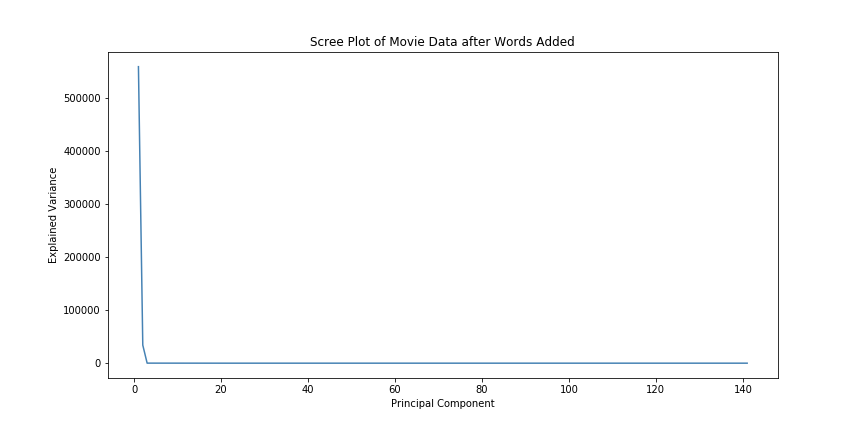
\includegraphics[width=\textwidth]{scree_whole}
\caption{\label{fig:scree_whole}Scree plot of principal components.}
\end{figure}

\begin{figure}%[H]
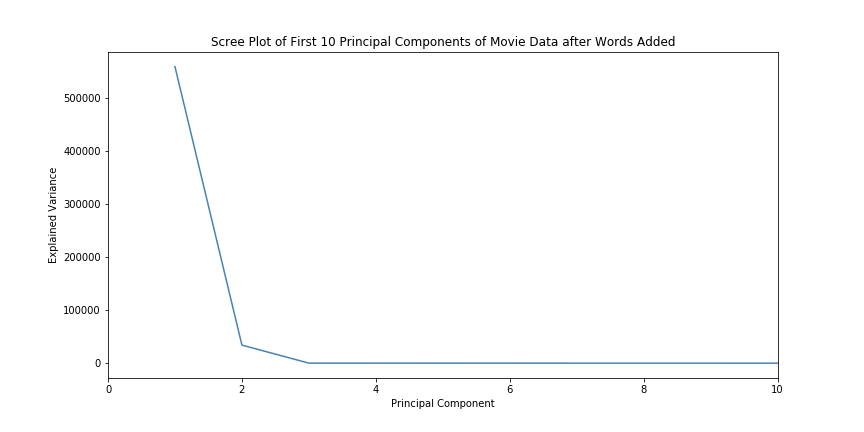
\includegraphics[width=\textwidth]{scree_first_10}
\caption{\label{fig:scree_first_10}Scree plot of first 10 principal components.}
\end{figure}

As Figure \ref{fig:pca_var_explained} shows, the first two princpal components account for almost 100\% of the variance in the dataset. The rotated data points are plotted along Princpal Components 1 and 2 in Figure \ref{fig:pc1_pc2}.

\begin{figure}%[H]
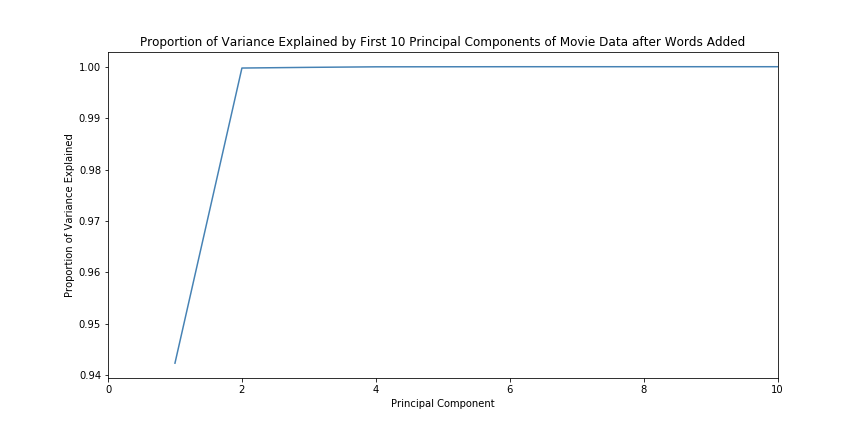
\includegraphics[width=\textwidth]{pca_var_explained}
\caption{\label{fig:pca_var_explained}Cumulative proportion of variance explained by first 10 principal components.}
\end{figure}

\begin{figure}%[H]
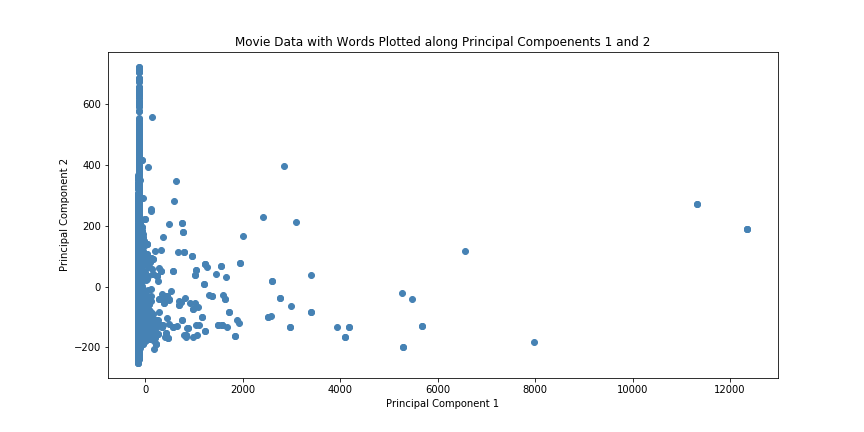
\includegraphics[width=\textwidth]{pc1_pc2}
\caption{\label{fig:pc1_pc2}Rotated data plotted along Princpal Components 1 and 2.}
\end{figure}

\subsection{Classification without Posters}
\label{section:class_no_posters_results}

After the first round of hyperparameter search, the ridge classifier performed best with $\alpha=0$, the support vector classifier with $C=100$, and the kNN classifier with 1 neighbor. The decision tree classifier had no hyperparameters of interest. The results of feature selection and tuning are provided in Table \ref{table:class_no_poster_results}. Table \ref{table:class_no_poster_test_results} details the testing MAE and RMSE for each model and feature selection scheme. The hyperparameters used in these models are:
\begin{itemize}
\item ridge: $\alpha=0$
\item SVC: $C=100$
\item kNN: 1 neighbor
\end{itemize}
The results show that a support vector classifier with $C=100$ and feature selection using mutual information is the best classifier, with an MAE of 0.87154 and an RMSE of 1.72500. The predictions of this classifier are depicted in Figure \ref{fig:no_poster_test_results}. This feature selection scheme chose 10 features: \texttt{popularity}, \texttt{vote\_count}, \texttt{Horror}, \texttt{Music}, \texttt{Thriller}, \texttt{overview\_len}, \texttt{day}, \texttt{take}, \texttt{direct}, and \texttt{evil}. The last three features correspond to the presence of words as described in \S \ref{section:words_results}.

\begin{table}
\resizebox{\textwidth}{!}{%
\begin{tabular}{l|ll|ll|l|ll}
\textbf{Classifier $\rightarrow$} & \textbf{Ridge} & \textbf{} & \textbf{SVC} & \textbf{} & \textbf{Decision Tree} & \textbf{kNN} & \textbf{} \\
\textbf{Feature Selection Scheme $\downarrow$} & \textbf{$\alpha$} & \textbf{MAE} & \textbf{$C$} & \textbf{MAE} & \textbf{MAE} & \textbf{neighbors} & \textbf{MAE} \\ \hline
\textbf{No Selection} & 0 & 1.19740 & 100 & 0 & 0 & 1 & 0 \\
\textbf{Chi-Squared Statistics} & 0.1 & 1.40022 & 10 & 0 & 0 & 1 & 0 \\
\textbf{ANOVA F-value} & 0 & 1.40130 & 100 & 1.15998 & 0.27983 & 1 & 0.32484 \\
\textbf{Mutual Information} & 0 & 1.41811 & 10 & 0 & 0 & 1 & 0
\end{tabular}%
}
\caption{\label{table:class_no_poster_results}Results of feature selection and hyperparameter tuning without posters.}
\end{table}

\begin{table}
\resizebox{\textwidth}{!}{%
\begin{tabular}{l|ll|ll|ll|ll}
\textbf{Classifier $\rightarrow$} & \textbf{Ridge} & \textbf{} & \textbf{SVC} & \textbf{} & \textbf{Decision Tree} & \textbf{} & \textbf{kNN} & \textbf{} \\
\textbf{Feature Selection Scheme $\downarrow$} & \textbf{MAE} & \textbf{RMSE} & \textbf{MAE} & \textbf{RMSE} & \textbf{MAE} & \textbf{RMSE} & \textbf{MAE} & \textbf{RMSE} \\ \hline
\textbf{No Selection} & 1.46016 & 2.14438 & 0.95772 & 1.80289 & 0.95610 & 1.94309 & 1.07805 & 1.94518 \\
\textbf{Chi-Squared Statistics} & 1.36260 & 1.98449 & 0.90569 & 1.76460 & 1.01789 & 2.01377 & 1.07967 & 1.96638 \\
\textbf{ANOVA F-value} & 1.38537 & 2.03386 & 1.43577 & 2.15836 & 1.14472 & 2.15271 & 1.18699 & 2.20421 \\
\textbf{Mutual Information} & 1.46992 & 2.04661 & 0.87154 & 1.72500 & 1.03089 & 1.96886 & 1.08618 & 1.96804
\end{tabular}%
}
\caption{\label{table:class_no_poster_test_results}Classifier testing errors on classification without posters.}
\end{table}

\begin{figure}%[H]
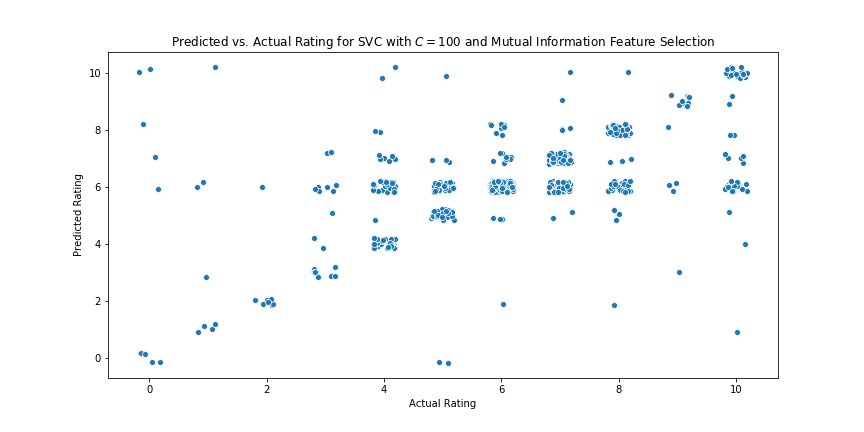
\includegraphics[width=\textwidth]{no_poster_test_results}
\caption{\label{fig:no_poster_test_results}Results of classification without posters with $U(-0.2, 0.2)$ jittering on both axes.}
\end{figure}

\subsection{Classifying Movie Posters}

This section created multiple neural networks, both convolutional and otherwise. The non-convolutional neural networks were trained on the flattened image arrays and contained different numbers dense hidden layers. Both softmax and sigmoid activation functions for the final layer were considered. The convolutional NNs were trained on the 3-dimensional image arrays, which were then flattened and run through non-convolutional dense layers. All NNs in this section use the Adam optimizer and categorical cross-entropy loss.

Several neural network models analyzes in this section predicted all fours or all zeros, including one of the convolutional NNs, defined in \texttt{keras} as below: \\
\texttt{%
model = Sequential()  \\
model.add(Conv2D(32, (2, 2), input\_shape=input\_shape))  \\
model.add(Activation('relu'))  \\
model.add(MaxPooling2D(pool\_size=(2, 2)))  \\
\\
model.add(Conv2D(32, (2, 2)))  \\
model.add(Activation('relu'))  \\
model.add(MaxPooling2D(pool\_size=(2, 2)))  \\
\\
model.add(Conv2D(64, (2, 2)))  \\
model.add(Activation('relu'))  \\
model.add(MaxPooling2D(pool\_size=(2, 2)))  \\
\\
model.add(Flatten())  \\
model.add(Dense(64))  \\
model.add(Activation('relu'))  \\
model.add(Dropout(0.5))  \\
model.add(Dense(dummy\_y.shape[1]))  \\
model.add(Activation('sigmoid')) \\
	\\
model.compile(loss="categorical\_crossentropy", optimizer="adam", \\
metrics=["mae", "mse"]) \\
} The testing prediction plot for this CNN is provided in Figure \ref{fig:cnn_all_fours}.

\begin{figure}%[H]
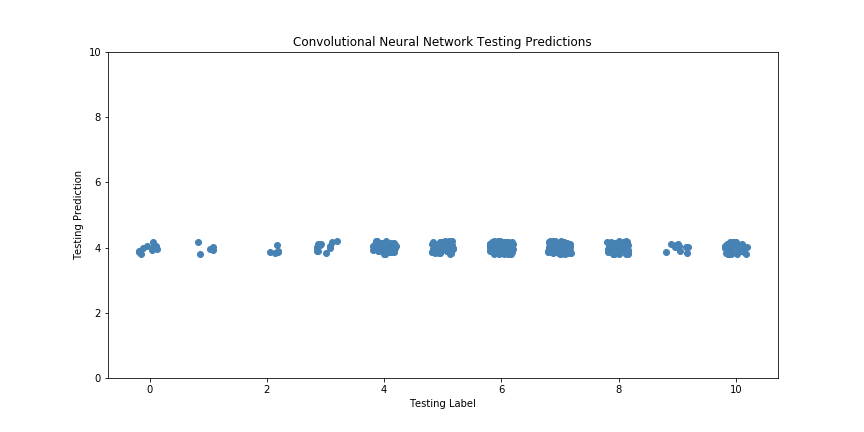
\includegraphics[width=\textwidth]{cnn_all_fours}
\caption{\label{fig:cnn_all_fours}Results of poster CNN with $U(-0.2, 0.2)$ jittering on both axes.}
\end{figure}

Several non-convolution neural networks were tested, including 11 non-convolutional fully-connected networks with 1 hidden layer trained over 100 epochs with batch size 16. The MAEs for these networks for different numbers of hidden units are provided in Table \ref{table:fcnn_maes}.

\begin{table}
\begin{center}\begin{tabular}{c|l}
\textbf{Number of Hidden Units} & \textbf{MAE} \\ \hline
1 & 1.989720549637178 \\
2 & 1.9078307858576502 \\
4 & 1.6101929905820598 \\
8 & 2.181723019916628 \\
16 & 1.712555195306469 \\
32 & 1.5834213370387524 \\
64 & 1.492082754361587 \\
128 & 1.492082754361587 \\
256 & 2.388825073336421 \\
512 & 2.0121877412382276 \\
1024 & 1.9250671607225567 \\
\end{tabular}\end{center}
\caption{\label{table:fcnn_maes}MAEs for different numbers of hidden units in non-convolutional fully-connected neural networks with 1 hidden layer.}
\end{table}

% \begin{appendices}
\newpage

\appendix
\section{Appendix: Word Signficiance Table}
\label{appendix:word_signif_table}

% TODO: move to appendix
\begin{table}[H]
\begin{tabular}[t]{l|l}
\textbf{Word}        & \textbf{p-value} \\ \hline
this        & 0.001    \\
after       & 0.006    \\
known       & 0.003    \\
% side        & 0.0      \\
killer      & 0.001    \\
business    & 0.019    \\
seem        & 0.009    \\
follows     & 0.028    \\
become      & 0.03     \\
house       & 0.003    \\
% meets       & 0.0      \\
aunt        & 0.017    \\
each        & 0.012    \\
making      & 0.001    \\
place       & 0.002    \\
% only        & 0.0      \\
foot        & 0.009    \\
% perform     & 0.0      \\
lore        & 0.036    \\
give        & 0.038    \\
found       & 0.031    \\
front       & 0.047    \\
women       & 0.024    \\
ours        & 0.035    \\
behind      & 0.001    \\
kill        & 0.004    \\
attempt     & 0.01     \\
disco       & 0.003    \\
mysterious  & 0.004    \\
king        & 0.015    \\
less        & 0.013    \\
turn        & 0.049    \\
begin       & 0.001    \\
years       & 0.002    \\
range       & 0.001    \\
discover    & 0.011    \\
\end{tabular}
\begin{tabular}[t]{l|l}
\textbf{Word}        & \textbf{p-value} \\ \hline
through     & 0.005    \\
take        & 0.012    \\
% group       & 0.0      \\
film        & 0.004    \\
gain        & 0.041    \\
% great       & 0.0      \\
trip        & 0.02     \\
care        & 0.009    \\
couple      & 0.049    \\
even        & 0.042    \\
party       & 0.027    \\
cove        & 0.003    \\
down        & 0.004    \\
% dire        & 0.0      \\
story       & 0.01     \\
father      & 0.04     \\
disc        & 0.009    \\
under       & 0.047    \\
ller        & 0.003    \\
busi        & 0.008    \\
direct      & 0.007    \\
light       & 0.002    \\
does        & 0.018    \\
dangerous   & 0.002    \\
break       & 0.007    \\
evil        & 0.005    \\
host        & 0.002    \\
survive     & 0.001    \\
meet        & 0.037    \\
realize     & 0.03     \\
% murder      & 0.0      \\
college     & 0.014    \\
documentary & 0.005    \\
self        & 0.02     \\
super       & 0.042    \\
across      & 0.006    \\
\end{tabular}
\begin{tabular}[t]{l|l}
\textbf{Word}        & \textbf{p-value} \\ \hline
rough       & 0.004    \\
cross       & 0.002    \\
hard        & 0.001    \\
brother     & 0.037    \\
childhood   & 0.001    \\
small       & 0.018    \\
director    & 0.02     \\
% feat        & 0.0      \\
danger      & 0.005    \\
dang        & 0.002    \\
between     & 0.003    \\
mean        & 0.003    \\
christmas   & 0.016    \\
year        & 0.018    \\
press       & 0.046    \\
ross        & 0.005    \\
dark        & 0.001    \\
% follow      & 0.0      \\
document    & 0.002    \\
% first       & 0.0      \\
brea        & 0.009    \\
anger       & 0.001    \\
strange     & 0.005    \\
hunt        & 0.002    \\
% secret      & 0.0      \\
takes       & 0.004    \\
fall        & 0.014    \\
% music       & 0.0      \\
which       & 0.029    \\
soon        & 0.002    \\
know        & 0.017    \\
% them        & 0.0      \\
wing        & 0.032    \\
% comedy      & 0.0      \\
form        & 0.001    \\
test        & 0.02     \\
cover       & 0.026    \\
mall        & 0.04     \\
\end{tabular}
\caption{\label{table:word_p_values}Words with statistically significant presences and corresponding p-values.}
\end{table}

% \end{appendices}

\end{document}